\documentclass[UTF8]{ctexbook}
%\includeonly{body/sta}

\usepackage[margin={2.5cm,1.5cm}]{geometry}

\usepackage{xcolor}
\usepackage[]{hyperref}
\usepackage{graphicx} % 用于插入图片(仿真展示可能用到)
\usepackage{caption} % 图片标题相关设置
\usepackage{subcaption} % 处理子图情况
\usepackage{makecell}
\usepackage{tikz}

\usepackage{amsmath} % 用于数学公式排版
\usepackage{amssymb} % 补充数学符号
\newcommand{\sgn}[1]{\mathop{\mathrm{sgn}} (#1)}
%\newcommand{\sig}[1]{\mathop{\mathrm{sig}} (#1)}
\newcommand{\sig}[1]{\lfloor #1 \rceil}
\usepackage{amsthm}
\newtheorem{theorem}{定理}
\newtheorem{definition}{定义}
\newtheorem{lemma}{引理}
\newtheorem{algo}{算法}
\newtheorem{proposition}{提案}
\newcommand\norm[1]{\left\lVert#1\right\rVert}
\newcommand\normx[1]{\Vert#1\Vert}
\newcommand{\NN}[0]{\mathbb{N}}
\newcommand{\RR}[0]{\mathbb{R}}

\newcommand{\Sgn}{\operatorname{Sgn}}
\newcommand{\sat}{\operatorname{sat}}
\newcommand{\diag}{\operatorname{diag}}
\newcommand{\dd}{\operatorname{d}}


 \usepackage[backend=biber, style=apa,url=false]{biblatex} % 指定后端为biber,引用样式为APA格式
%\addbibresource{main_biber.bib} 
 \addbibresource{biblatex.bib} 

\newcommand{\citefrom}[1]{\textcolor{gray}{#1}\\}
\newcommand\tR{\textcolor{red}}
\newcommand\tB{\textcolor{blue}}
\newcommand\tG{\textcolor{green}}

\title{滑模控制学习笔记}
\author{\href{mailto:xsro@foxmail.com}{xsro@foxmail.com} \href{https://xsro.github.io/about/}{xsro.github.io}}
\date{\today}

\begin{document}
	

	\maketitle
	\tableofcontents
	
	\chapter{前言}

非线性动态系统理论是滑模控制的重要理论基础,也是我学习滑模的最大障碍。
我决定花一些时间从工科本科数学知识出发整理非光滑(非连续)动态系统中的一些概念。
这篇笔记主要回顾连续性的定义,同时介绍传统的连续可微的classical解在应对非连续系统时存在性与唯一性的缺陷。

\section{引子}

最近在看滑模控制的文章,其中对于非连续系统的论述多有不解,比如如下Filippov微分包含到底是什么,比如我总是可以看到Filippov 这个定义,但是却对里面的数学分析、控制理论术语一窍不通。
\begin{quote}
  Filippov 微分包含的解的所有广为人知的性质(existence,extendability
  etc)但是不包含唯一性(uniqueness)。
\end{quote}
因此,我决定参考网络上的一些资料
\begin{enumerate}
  \item
    知乎讨论:请问filippov解大概是什么意思?是怎么定义的?有什么作用?
    \url{https://www.zhihu.com/question/55951952} 文中推荐参看\cite{cortesDiscontinuousDynamicalSystems2008,hanTheoryControlSystems2016}
  \item
\end{enumerate}
以及我检索到的一些文献,做一个简单的梳理。
本文主要是翻译自\cite{cortesDiscontinuousDynamicalSystems2008}。

\section{符号约定}

\subsection{分数幂奇函数}
本文常用的符号为符号函数和sig 函数,对于标量,其几何意义为符号函数,对于标量其定义为:
\begin{equation}
    \sig{x}^0=\sgn{x}=\begin{cases}
    	1   & x>0\\
    	-1 & x<0\\
    	0  & x=0\\
    \end{cases}
\end{equation}
基于此,我们定义$\sig{x}^q=|x|^q \sgn{x}$.

类似的,相关定义可以拓展到向量形式,其几何意义为向量$\vec{x}$的单位向量:
\begin{equation}
	\sig{\vec{x}}^0=\sgn{\vec{x}}=\begin{cases}
		\frac{\vec{x}}{\norm{\vec{x}}}, & \norm{\vec{x}}\neq 0\\
		\vec{0}   & \norm{\vec{x}}=0
	\end{cases}
\end{equation}
基于此,我们定义$\sig{\vec{x}}^q=\|\vec{x}\|^q \sgn{\vec{x}}$.

下面介绍对几个常见的求导运算,使用多维向量的情况。
\begin{equation}
	\frac{\dd}{\dd t} \norm{\vec{x}}
	= \frac{\dd}{\dd t} \sqrt{\vec{x}^T\vec{x}}
	= \frac12 \frac{1}{\sqrt{\vec{x}^T\vec{x}}}\frac{\dd}{\dd t} {\vec{x}^T\vec{x}}
	= \frac12 \frac{1}{\sqrt{\vec{x}^T\vec{x}}} (2 \vec{x}^T \dot{\vec{x}})
	= \frac{\vec{x}^T\dot{\vec{x}}}{\norm{\vec{x}}}
\end{equation}
\begin{equation}
	\frac{\dd}{\dd t} \sig{\vec{x}}^q
	=\frac{\dd}{\dd t} \norm{\vec{x}}^{q-1} \vec{x}
	=\norm{\vec{x}}^{q-1} \dot{\vec{x}}+(q-1) \norm{\vec{x}}^{q-2}  \frac{\vec{x}^T\dot{\vec{x}}}{\norm{\vec{x}}}\vec{x}
\end{equation}
也就是说这里是基于向量的定义是难以求导的,这给一些从标量系统到向量的分析带来了困难。
\begin{equation}
	\frac{\dd}{\dd t} \sig{x}^q
	=|x|^{q-1} \dot{x}+(q-1) |x|^{q-2}  \frac{x \dot{x}}{|x|}x
	=q|x|^{q-1}\dot{x},
\end{equation}


\begin{figure}
	\centering
	\begin{tikzpicture}
		\draw[->] (-2.2,0) -- (2.2,0) node[right] {$x$};
		\draw[->] (0,-1.8) -- (0,2.2) node[above] {$y$};
		\draw[domain=0:1.3,smooth,variable=\x,blue] plot ({\x},{\x*\x}); 
		\draw[domain=-1.3:0,smooth,variable=\x,blue] plot ({\x},{-\x*\x}); 
		\node[blue] at (2,2) {$y_1=\sig{x}^2$};
		\draw[domain=0:1.4,smooth,variable=\x,cyan] plot ({\x},{sqrt(\x)}); 
		\draw[domain=-1.4:0,smooth,variable=\x,cyan] plot ({\x},{-sqrt(-\x)}); 
		\node[cyan] at (2.4,1) {$y_2=\sig{x}^{1/2}$};
	\end{tikzpicture}
	\quad
	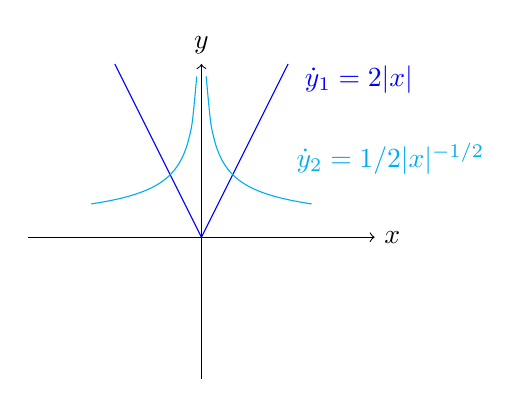
\begin{tikzpicture}
		\draw[->] (-2.2,0) -- (2.2,0) node[right] {$x$};
		\draw[->] (0,-1.8) -- (0,2.2) node[above] {$y$};
		\draw[domain=0:1.1,smooth,variable=\x,blue] plot ({\x},{2*\x}); 
		\draw[domain=-1.1:0,smooth,variable=\x,blue] plot ({\x},{-2*\x}); 
		\node[blue] at (2,2) {$\dot{y}_1=2|x|$};
		\draw[domain=0.06:1.4,smooth,variable=\x,cyan] plot ({\x},{1/2*1/sqrt(\x)}); 
		\draw[domain=-1.4:-0.06,smooth,variable=\x,cyan] plot ({\x},{1/2*1/sqrt(-\x)}); 
		\node[cyan] at (2.4,1) {$\dot{y}_2=1/2|x|^{-1/2}$};
	\end{tikzpicture}
	\caption{两个分数幂函数及其导数}
\end{figure}




\section{回顾:连续性}\label{ux56deux987eux8fdeux7eedux6027}

那么什么是Lipschitz连续呢,各种连续的关系又是什么呢,我们讨论的非连续动态微分方程又如何定义呢?
为了简便,这里用的是函数来叙述,实际控制理论中大多为多维到多维的向量函数。如果是多变量函数或者泛函需要使用范数替代绝对值。

可微必可导。
可微是可导的充分条件。
只不过在一元情况下,由于两点确定一条直线,导致可微的线性替代就相当于求导(斜率确定 点确定 相当于直线确定)

\subsection{点连续与间断点}

\begin{definition}[点连续]
设函数\(y=f(x)\)在点\(x_0\)的某一邻域内有定义,
并且\(\lim_{x\to x_0}f(x)=f(x_0)\),
那么就称函数\(f(x)\)在点\(x_0\)处连续。
\end{definition}

借此可以定义函数不连续和间断点的概念:
\begin{definition}
设函数\(f(x)\)在点\(x_0\)的某\textbf{去心}领域内有定义,
在此前提下,如果函数\(f(x)\)有一下三种情形之一 
\begin{enumerate}
  \item 在\(x=x_0\)处没有定义;
  \item 在\(x=x_0\)处有定义,但\(\lim_{x\to x_0} f(x)\)不存在;
  \item 在\(x=x_0\)处有定义,\(\lim_{x\to x_0} f(x)\)存在,但\(\lim_{x\to x_0}\neq f(x_0)\)
\end{enumerate}
那么函数\(f(x)\)在点\(x_0\)为不连续,\(x_0\)是函数\(f(x)\)的\textbf{间断点}。
\end{definition}



函数的间断点可以分为 
\begin{enumerate}
  \item 第一类间断点:左右极限都存在 
  \begin{enumerate}
    \item 可去间断点:左右极限都存在且相等 
    \item 跳跃间断点:左右极限都存在但不等 
  \end{enumerate}
  \item 第二类间断点:左右极限至少有一个不存在 
  \begin{enumerate}
    \item 震荡间断点:\(\lim_{x\to\ x_0} f(x)\)振荡不存在 
    \item 无穷间断点:\(\lim_{x\to\ x_0^+} f(x)=\infty\)或\(\lim_{x\to\ x_0^-} f(x)=\infty\)
  \end{enumerate}
\end{enumerate}


\begin{figure}[!hbp]
\centering
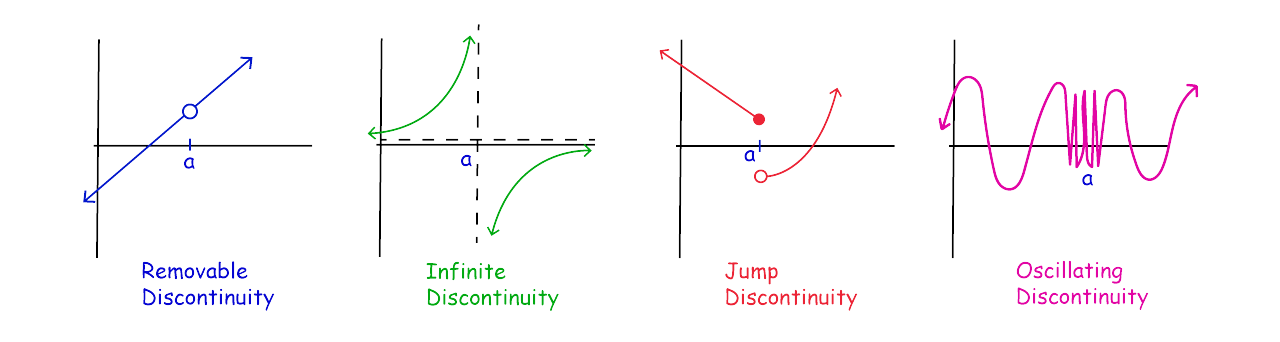
\includegraphics[width=\linewidth]{asserts/4-types-of-discontinuity.png}
\caption{
  间断点的定义与图示(来源:\url{https://calcworkshop.com/limits/limits-and-continuity/})
}
\end{figure}

\subsection{区间连续与区间一致连续(连续、绝对连续、Lipschitz连续、Hölder连续)}

如果在区间上每一点都连续,就称函数在该区间上连续,如果区间包括端点,那么在右端点连续是指左连续,在左端点连续是指右连续。

\begin{definition}[区间连续]
设函数\(f(x)\)在区间\(I\)上有定义.
如果对于任意给定的正数\(\epsilon\),总存在正数
\(\delta\),是的对于区间\(I\)上的任意两点\(x_1,x_2\),当\(|x_1-x_2|<\delta\)时,
有 \[
|f(x_1)-f(x_2)|<\epsilon
\] 那么称函数\(f(x)\)在区间\(I\)上\textbf{一致连续}。
\end{definition}

绝对连续表示函数的光滑性质,比连续和一致连续条件都要严格,比Lipschitz条件宽松,是一类极为重要的函数。绝对连续函数几乎处处可微,是它的导函数的广义原函数。

\begin{definition}[绝对连续]
设\(f(x)\)是\([a,b]\)上的函数,若对任意\(\epsilon>0\),存在\(\delta>0\)使得对于
\([a,b]\)中的任意一组分点: \[
a_1<b_1\leq a_2 <b_2 \leq \dots \leq a_n < b_n,
\] 只要\(\sum_{i=1}^n(b_i-a_i)<\delta\),便有 \[
\sum_{i=1}^n|f(b_i)-f(a_i)|<\epsilon
\]
则称\(f(x)\)是\([a,b]\)上\textbf{绝对连续}函数,或称\(f(x)\)在\([a,b]\)上绝对连续。
\end{definition}

等价的,如果存在一个Lebesgue可积函数\(\kappa:[a,b]\to \mathbb{R}\)
使得下式成立,那么\(\gamma\)是一个绝对连续函数。 \[
\gamma(t)=\gamma(a)+\int^t_a \kappa(s)d s,\quad t\in [a,b]
\]

\begin{definition}[Lipschitz连续]
对于函数\(f(x)\),如果存在一个常数L,使得对\(f(x)\)定义域上(可为实数也可以为复数)的任意两个值满足如下条件:
\[
|f(x_1)-f(x_2)|\leq L|x_1-x_2|
\]
那么称函数\(f(x)\)满足Lipschitz连续条件,并称L为\(f(x)\)的lipschitz常数。
\end{definition}

\begin{itemize}

\item
  从局部看:我们可以取两个充分接近的点,如果这个时候斜率的极限存在的话,这个斜率的极限就是这个点的导数。也就是说函数可导,又是Lipschitz连续,那么导数有界。反过来,如果可导函数,导数有界,可以推出函数Lipschitz连续。
\item
  从整体看:Lipschitz连续要求函数在无限的区间上不能有超过线性的增长,所以这些x\textsuperscript{\{2\}和e}\{2\}函数在无限区间上不是Lipschitz连续的。
\end{itemize}

\begin{quote}
对于函数\(f(x)\),如果存在一个非负常数\(C,\alpha\),
使得对\(f(x)\)定义域上(可为实数也可以为复数)的任意两个值满足如下条件:
\[
|f(x_1)-f(x_2)|\leq C|x_1-x_2|^\alpha
\] 那么称函数\(f(x)\)满足Hölder连续条件。
当\(\alpha=0\)时表示有界,当\(\alpha=1\)时表示满足Lipschitz条件
\end{quote}

\subsection{区间上连续性的关系}\label{ux533aux95f4ux4e0aux8fdeux7eedux6027ux7684ux5173ux7cfb}

图\ref{fig continuity}刻画了控制理论中常用的连续性的关系,我们也可以举出常见的反例。

\begin{table}\centering
  \begin{tabular}{c|c|c}
    一直连续但是不绝对连续 & 
    \(
      f_1(x)=\begin{cases}
        0, &x=0\\
        x \sin\frac{\pi}{x}, &0 < x\leq 1
      \end{cases}
    \)& 
    \\\hline
    绝对连续但是不Lipschitz连续&
    \(f_3(t)=\sqrt{|t|},t\in [-1,1]\)&
    绝对连续但是在0处不Lipschitz连续
    \\\hline
    Lipschitz连续但是不可导&
    \(f(t)=|t|,t\in[-1,1]\)&
    在0处局部Lipschitz但在零处不可导\\
  \end{tabular}
\end{table}

\begin{figure}[!htp]\centering
  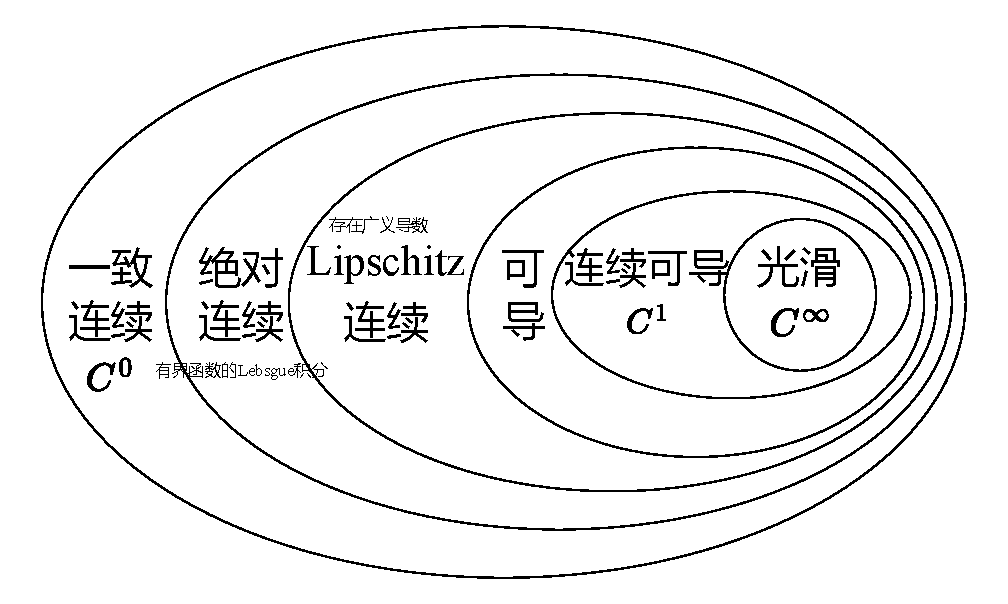
\includegraphics[width=0.6\linewidth]{asserts/连续的关系.drawio.pdf}
  \caption{控制理论中常用的连续性质的关系}
  \label{fig continuity}
\end{figure}


如下绝对值函数\(f_2(x)\)绝对连续但是在0处不连续可微 \[
f_2(x)=|x|, x\in [-1,1]
\]

如下根号函数绝对连续但是在0处不是局部Lipschitz连续的 \[
f_3(t)=\sqrt(t),t\in [0,0]
\]

\section{连续可微和光滑}

连续可微(Continuously differentiable),用泛函表示就是函数\(f\in C^1\),意味着函数的导数是连续的,当然可微保证其本身也是连续的。

光滑函数(英语:Smooth function)在数学中特指无穷可导的函数,不存在尖点,也就是说所有的有限阶导数都存在。例如,指数函数就是光滑的,因为指数函数的导数是指数函数本身。

\begin{definition}[光滑函数]
  若一函数是连续的,则称其为\(C^{0}\)函数;
  若函数存在导函数,且其导函数连续,则称为连续可导,记为\(C^1\)函数;
  若一函数n阶可导,并且其n阶导函数连续,则为\(C^{n}\)函数(\(n\geq 1\))。
  而光滑函数是对所有n都属于\(C^{n}\)函数,特称其为\(C^{\infty }\)函数。
\end{definition}


\section{内容概要}

从这个图可以看出在经典解中解$x(t)$是$f(x(t))$的积分,而Filippov解中$x(t)$是$f(x(t))$的Lebsgue积分。
经典解中的解是连续可导的,连续可导的意思是可导并且其导数连续,这与存在性条件$f(x(t))$连续一致。
类似地,Filippov解中解是绝对连续的,这与存在性条件$f(x(t))$可测并且局部本质有界一致。

\begin{table}[!htp]
  \centering
  \begin{tabular}{|c|c|c|c|}
    \hline
    & 解$x(t)$的连续性 & 存在性条件 & 唯一性条件 \\\hline
    经典解 & 连续可导 & 
    $f(x)$连续 & $f(x)$ Lipschitz连续\\\hline
    Filippov解 & 绝对连续 & 
    $f(x)$ 可测并且局部本质有界 & $f(x)$ Lipschitz连续 \\\hline
  \end{tabular}
  \caption{微分方程$\dot{x}=f(x)$Filippov解}
\end{table}

Every vector field that is locally Lipschitz at $x$ satisfies the one-sided Lipschitz condition on a neighborhood of $x$, but the converse is not true.





	\chapter{非线性系统:右端Lipschtz连续}

一般的非线性自治系统可以用如下方程表示:
\begin{equation}\label{eq:nonlinear}
    \dot{x}=f(t,x).
\end{equation}
其中,$x$为系统状态,$t\geq 0$为时间。
$f(t,x)$ 是关于时间$t$分段连续的,关于状态$x$是局部Lipschitz连续的。
is \strong{piecewise continuous in $t$} and \strong{locally Lipshitz in $x$} over the domain of interest


经典非线性系统的解存在性和唯一性需要微分方程右端Lipschitz连续,
一个使用较多的数学表述是khalil的非线性控制的\textbf{引理1.3}:

\begin{quote}
设\(f(t,x)\)关于\(t\)是\textbf{分段连续}的,
并且对所有\(t\ge t_0\),在关于\(x\)的区域\(D\subset \mathbb{R}^n\)上\(f(t,x)\)是局部\textbf{Lipschitz连续}的。
设\(W\)是\(D\)中的一个紧子集,\(x_0\in W\),并进一步设 \[
\dot{x}=f(t,x),x(t_0)=x_0
\] 的解\(t\ge t_0\)时都在\(W\)内,那么这个解是\(t\ge t_0\)的唯一解。
\end{quote}

    $f(t,x)$ is piecewise continuous in $t$ on interval $J\subset \RR$ 
    if for every bounded subinterval $J_0\subset J$, 
    $f$ is continuous in $t$ for all $t\in J_0$, 
    except, possibly, 
    at a finite number of points where $f$ may have finite-jump discontinuities.

    $f(t,x)$ is \textcolor{blue}{locally Lipschitz} in $x$ \textcolor{red}{at a point $x_0$} 
    if there is a neighborhood $N(x_0,r)=\{x\in \RR^n \big| \norm{x-x_0}<r\}$ 
    where $f(t,x)$ satisfies the Lipschitz condition
    \[\norm{f(t,x)-f(t,y)}\le \norm{x-y},L>0\] 

    A function $f(t,x)$ is \textcolor{blue}{locally Lipschitz} in $x$ 
    \textcolor{purple}{on a domain} (open and connected set) $D\subset\RR^n$ 
    if it is locally Lipschitz at every point $x_0\in D$

    \begin{lemma}[lemma 1.1 \cite{khalilNonlinearControl2015}]
        Let $f(t,x)$ be piecewise continuous in $t$ and \strong{locally} Lipschitz 
        in $x$ at $x_0$,
        for all $t\in [t_0,t_1]$.
        Then, there is $\delta >0$ such that the state equation $\dot{x}=f(t,x)$,
         with $x(t_0)=x_0$,
        has a unique solution over $[t_0,t_0+\delta]$.
    \end{lemma}

    \begin{lemma}[lemma 1.3]
        Let $f(t,x)$ be piecewise continuous in $t$ and 
        \strong{locally Lipschitz} in $x$ for all $t\in [t_0,\infty)$
        and all $x$ in a domain $D\subset \RR^n$.
        Let $W$ be a compact subset of $D$, 
        and suppose that every solution of 
        \[\dot{x}=f(t,x), x(t_0)=x_0\]
        with $x_0\in W$ lies entirely in $W$. 
        Then, there is a unique solution that is defined for all $t\ge t_0$
    \end{lemma}

    \begin{theorem}[Lyapunov's theorem (3.3)]
        If there is $V(x)$ such that 
            \begin{itemize}
                \item[1] $V(0)=0$
                \item[2] $V(x)>0, \ \forall \ x \in D \ with\ x\neq 0$
                \item[3] $\dot{V}(x) \le 0, \forall\ x\in D$
            \end{itemize}
            then the origin is \strong{stable}

        Moreover, If 
        \[\dot{V}(x)<0,\ \forall \ x\in D \ with\ x\neq 0\]
        then the origin is \strong{asymptotically stable}

        Furthermore, if $V(x)>0, \forall \ x\neq 0$,
        \[\norm{x}\to \infty \rightarrow V(x) \to \infty\]
        and $\dot{V}(x)<0,\forall\ x\neq 0$, then the origin is \strong{globally asymptotically stable}
    \end{theorem} 

    \begin{theorem}[Lyapunov's Theorem]
        The origin is stable if there is a continuously differentiable positive definite function $V(x)$ so that $\dot{V}(x)$ is negative definite. 
        It is globally asymptotically stable if the conditions for asymptotic stable hold globally and ${V}(x)$ is radially unbounded.
    \end{theorem}
    \chapter{连续控制系统}


\section{非光滑Lyapunov 方法(Dini导数)}

使用Dini导数表示的非光滑系统李亚普诺夫方法见书\cite{roucheStabilityTheoryLiapunov1977}。
Dini导数可以用于计算连续但是不可导的函数的导数,因此常用于非光滑系统的分析。
Dini导数的定义为:

\begin{definition}[Dini导数]
  \citefrom{\cite[p 659 in proof of theorem 3.4]{khalilNonlinearSystems}}
  The \textbf{upper Dini derivative}, which is also called an upper right-hand derivative, of continuous function  is defined by 
  \begin{equation}
    D^+ v(t) = \limsup_{h\to 0^+} \frac{v(t+h)-v(t)}{h}
  \end{equation}
  where $\limsup_{n\to\infty}$ (the limit superior).
\end{definition}
这里的$\limsup$是上极限,形象地理解是,函数$y=\sin(x)$在无穷处是没有极限的,但是在无穷远处是有上极限$\limsup_{x\to\infty} \sin(x)=1$和下极限$\liminf_{x\to\infty} \sin(x)=-1$的。

\begin{lemma}[非光滑版本的 LaSalle 不变集原理]
  \citefrom{最早出自\cite[Theorem 2]{lasalleStabilityTheoryOrdinary1968}
  也见于\cite[p 243]{roucheStabilityTheoryLiapunov1977}}
  % yuSecondorderConsensusMultiagent2017
  Let $x(t)$ be a solution of $\dot{x} = f(x)$ with $x(0) = x_0 \in \RR^k$, where \tR{$f: U \to \RR^k$ is continuous} with an open subset $U$ of $R^k$, and let $V: U \to R$ be a locally Lipschitz function such that $D^+V(x(t)) ≤ 0$, where $D^+$ denotes the upper Dini derivative. 
  Then, with denoting the positive limit set as $\lambda^+(x_0)$, $\lambda^+(x_0)\cup U$ is contained in the union of all solutions that remain in $S = \{x \in U : D^+V(x(t)) = 0\}$.
\end{lemma}
    \chapter{非光滑控制系统:右端有界}

对于右端不连续的系统,目前仍然是学界的研究重点,主流有两种方法来刻画(\cite{poznyakVadimUtkinSliding2023})。
一个是以\cite{filippovDifferentialEquationsDiscontinuous1988}为代表的Filippov方法,一个是Utkin的equivalent control (EC)方法。
其余方法可以见短文\cite{utkinBriefCommentsDoubts2022}、杂志\cite{cortesDiscontinuousDynamicalSystems2008}等文献。

\section{不一定连续可微的解}



考虑如下的动态系统 \[
\dot{x}(t)=\mathcal{X}(x(t))\ x(t_0)=x_0
\tag{7}
\] 其中\(x\in \mathbb{R}^d\), \(d\)为一个正整数,
并且\(\mathcal{X}:\mathbb{R}^d \to \mathbb{R}^d\) \textbf{不需要连续}。
我们称\textbf{连续可微的解\(t \mapsto x(t)\)为经典(classical)解}。
显然,如果\(\mathcal{X}\)连续,那么方程所有解都是classical的。
不失一般性,我们认为\(t_0=0\),并且只考虑\(t>0\)的情况。



\textbf{Caratheodory解}是classical解的一般化。
粗略地说,Caratheodory解是满足微分方程(7)的Lebesgue积分形式(8)的绝对连续曲线
\[
x(t)=x(t_0)+\int_{t_0}^t X(x(s)) ds,\quad t>t_0
\tag{8}
\]
通过使用积分形式(8),Caratheodory解不再要求方程解必须所有时间都沿着向量场的方向。
也就是说,微分方程(7)need bot be satisfied on a set of measure zero.

\textbf{Filippov解}使用微分包含式(differential
inclusion)来替换微分方程(7)右侧 \[
\dot{x}(t)\in \mathcal{F} (x(t))
\] 其中\(\mathcal{F}:\mathbb{F}^d \to \mathfrak{B}(\mathbb{F}^d)\),
\(\mathfrak{B}(\mathbb{R}^d)\)为d维实数空间\(\mathbb{R}^d\)的所有子集的集合。
Filippov解是绝对连续曲线。
对于任意给定的状态\(x\),Filippov解不只关注向量场在\(x\)处的值,
Filippov解的思想是引入由向量场中\(x\)的领域决定的一组\textbf{方向集合}。
文献中常常使用集值映射(set-value map),
也就是说这种映射的值是一个集合,而不像标准的函数(映射)的值只有一个。

\begin{quote}
An ordinary differential inclusion says the derivative must lie in a
specified set, which may also depend on the function and independent
variable.
\end{quote}

Caratheodory解和Filippov解都不能完全解决非连续动态系统的问题,
围绕存在的问题由\textbf{Sample-and-hold}解以及其他的一些描述方法。

\subsection{解的存在性和唯一性}\label{ux89e3ux7684ux5b58ux5728ux6027ux548cux552fux4e00ux6027}

对于常微分方程而言,向量场如果只连续不能保证解的唯一性。
我们说解的一个性质弱,表示不是所有解满足这一性质。
我们说解的一个性质强,表示所有解满足这一性质。
所以设计控制器的思路可以是

\begin{enumerate}
\def\labelenumi{\arabic{enumi}.}

\item
  设计控制器并考虑控制器下的闭环系统
\item
  用一个集值映射将每一个状态映射到允许的输入产生的所有向量的集合,并将这个映射与控制系统关联起来,(原文表述如下)
\end{enumerate}

\begin{quote}
associate with the control system the set-valued map that assigns each
state to the set of all vectors generated by the allowable inputs and
consider the resulting differential inclusion.
\end{quote}

\subsection{classical
解的存在性}\label{classical-ux89e3ux7684ux5b58ux5728ux6027}

考虑微分方程: \[
\dot{x}(t)=X(x(t)),\quad x(0)=x_0
\tag{10}
\] 其中\(X:\mathbb{R}^d \to \mathbb{R}^d\)是一个向量场。
如果\(0=X(x_e)\),那么点\(x_e\in \mathbb{R}^d\)是(10)的一个平衡点。
在\([0,t_1]\)上一个(10)的classical解是一个连续可微的映射\(x:[0,t_1]\to\mathbb{R}^d\)。
不失一般性,我们只考虑从时间\(t_0=0\)开始的解。 如果解\(t\mapsto x(t)\)
不能在时间上延申(extend),
也就是说解不是定义域内更大的一个时间区间上的解的截断,
那么称该解为最大解(maximal solution)。
最大解的定义暗示了解的区间只能是\([0,T),T>0\)或\([0,\infty)\)。

Peano's theorem 说明了连续的向量场可以保证classical解存在:

\begin{quote}
(Proposition 1) 令\(X:\mathbb{R}^d\to \mathbb{R}^d\)是连续向量场。
于是,对于所有\(x_0\in\mathbb{R}^d\),
\textbf{存在}一个(10)的classical解,该解满足\(x(0)=x_0\)
\end{quote}

\subsection{classical
解的唯一性}\label{classical-ux89e3ux7684ux552fux4e00ux6027}

\begin{quote}
(Proposition 2) 令\(x:\mathbb{R}^d\to\mathbb{R}^d\)连续,
假设对于所有的\(x\in\mathbb{R}^d\),
存在一个\(\epsilon>0\)使得\(X\)是在状态\(x\)的\(\epsilon\)领域\(B(x,\epsilon)\)上单侧Lipschitz连续。
然后,对于所有\(x_0\in \mathbb{R}^d\),存在一个起始于\(x(0)=x_0\)的(10)的\textbf{唯一的}classical
解
\end{quote}

\subsection{classical
解存在性和唯一性示例}\label{classical-ux89e3ux5b58ux5728ux6027ux548cux552fux4e00ux6027ux793aux4f8b}

下面的例子说明如果向量场不连续,那么(10)可能不存在经典解

\begin{quote}
考虑如下向量场:\(X:\mathbb{R}\to\mathbb{R}\) \[
X(x)=\begin{cases}
-1, & x>0\\
1 , & x\leq 0
\end{cases}
\] 显然在\(x=0\)处该函数不连续。
假设存在一个连续可微的解满足\(\dot{x}(t)=X(x(t))\)和\(x(0)=0\)。
然后\(\dot{x}(0)=X(x(0))=X(0)=1\),
于是,对于所有的充分小的时间\(t\),\(x(t)>0\)
并且\(\dot{x}(t)=X(x(t))=-1\), 这与\(t\mapsto \dot{x}(t)\)连续矛盾。
所以,不存在classical 解。
\end{quote}

下面的例子说明如果向量场不连续,那么(10)也可能存在经典解。

\begin{quote}
考虑向量场\(X:\mathbb{R}\to\mathbb{R}\) \[
X(x)=-\mathrm{sign}(x)=\begin{cases}
-1, & x>0,\\
0,   & x=0,\\
1,   & x<0,
\end{cases}
\] 唯一最大解为: \[
\begin{aligned}
&x(t)=x(0)-t, 
t\in [0,x(0)) 
&\textrm{if}
\ x(0)>0, \\
&x(t)=0,  t\in [0,\infty)
&\textrm{if}\ x(0)=0 
\\
&x(t)=x(0)+t,  t\in [0,-x(0))
&\textrm{if}\ 
x(0)<0,
\end{aligned}
\]
\end{quote}

下面例子说明连续但是不是单侧Lipschitz连续的向量场可能有多个classical解

\begin{quote}
考虑向量场\(X:\mathbb{R}\to\mathbb{R}\) \[
X(s)=\sqrt{|x|}
\] 这个向量场处处连续,并在\(\mathbb{R}/\{0\}\)局部Lipschitz连续,
但是在零处不局部连续,在零的领域也不单侧Lipschitz连续。
从\(x(0)=0\)开始,该动态系统有许多最大解,具体而言为:
对所有\(a>0\),\(x_a:[0,\infty)\to \mathbb{R}\),表达式为: \[
x_a(t)=\begin{cases}
0, & 0\leq t \leq a,\\
(t-a)^2/4, & t\geq a
\end{cases}
\]
\end{quote}

下面例子说明连续但是不是单侧Lipschitz连续的向量场只有一个classical解
\textgreater{} 考虑向量场\(X:\mathbb{R}\to\mathbb{R}\) \[
X(s)=\begin{cases}
-x \mathrm{log} x, & x>0\\
0,                            & x=0,\\
x \mathrm{log}(-x),& x<0,
\end{cases}
\] \textgreater{} 唯一最大解为: \[
\begin{aligned}
    &x(t)=-\exp(\log (-x(0)) \exp(t)), 
    &\textrm{if}\ x(0)<0 \\
    &x(t)=0, 
    &\textrm{if}\ x(0)=0 \\
    &x(t)=\exp(\log x(0) \exp(-t)), 
    &\textrm{if}\ x(0)>0
\end{aligned}
\]



\section{非光滑Lyapunov 方法(chark梯度)}


本节参照\parencite{shevitzLyapunovStabilityTheory1994,郑凯_基于Filippov微分包含解的非平滑控制系统},介绍非光滑微分方程Filippov解的定义及其稳定性的基本定理。

考虑向量微分方程
\begin{equation}\label{eq:nonsmooth diff}
    \dot{x}=f(x,t)
\end{equation}
其中函数 $f:\RR^p \times \RR \to \RR^p$ 是可测的(measurable),并且满足局部本性有界(essentially locally bounded)。
首先定义该方程的解。

\begin{definition}
    (Filippov解,\cite{filippovDifferentialEquationsDiscontinuous1988})
    如果一个关于时间$t$的函数$x(t)$在$[t_0,t_1]$上绝对连续,并且对于几乎(almost)所有$t\in[t_0,t_1]$满足
    \[
        \dot{x}\in \mathbb{K}[f](x,t),
        \quad 
        \mathbb{K}[f](x,t)=\bigcap_{\delta>0} \bigcap_{\mu(\bar{N})=0} \overline{co} f(B(x,\delta)\backslash \bar{N},t)
    \]
    那么称该函数$x(t)$为\eqref{eq:nonsmooth diff}的解。
    这里,
    $\bigcap_{\mu(\bar{N})=0}$表示所有Lebesgue测度为0的集合$\bar{N}$的交集,
    $\overline{co}(X)$表示$X$的凸闭包,$B(x,\delta)$表示以$x$为球心,$\delta$为半径的开球。
\end{definition}

\subsubsection{广义梯度与广义微分}

广义梯度和广义微分都是针对Lipschitz连续函数的,Lipschitz连续是连续的一种特殊情况。

\begin{definition}[广义方向导数]\cite{clarkeOptimizationNonsmoothAnalysis1990}
    若函数$V:\Omega\to\RR$在$x$附近是Lipschitz连续的,向量$v\in\Omega$,则函数$V$在$x$处沿$v$方向的广义方向导数为
    \begin{equation}
        V^o(x;v)=
        \limsup_{y\to x ,h\downarrow 0} 
        \frac{V(y+hv)-V(y)}{h}
    \end{equation}
    其中$y\in\Omega$.
\end{definition}
这里的广义方向导数在$x$处是关于$v$的正齐次可加函数,可作为支持函数确定一凸集\cite{clarkeOptimizationNonsmoothAnalysis1990},我们将这一凸集定义为函数$f(x)$在$x$处的广义梯度。

\begin{definition}[广义梯度]\cite{clarkeOptimizationNonsmoothAnalysis1990}
    若函数$V:\Omega\to\RR$在$x$附近是Lipschitz连续的,则函数$f$在$x$处的广义梯度定义为
    \begin{equation}
        \partial V(x)=
        \{\zeta \in\RR^n \big|  
        V^o(x;v)\geq \langle\zeta,v\rangle, \forall v\in\Omega\}
    \end{equation}
\end{definition}

\begin{theorem}[广义梯度的计算]
    \cite{clarkeOptimizationNonsmoothAnalysis1990}
    \label{thm:general gradient}
    对于一个局部Lipschitz连续的函数$V:\RR^p\times \RR\to \RR$,
    定义
    \begin{equation}
        \label{eq:general gradient}
        \partial V(x,t)=\overline{co}\{\lim_{y\to x}\nabla V(x)|
        y\notin S,
        y\notin \Omega_f\}
    \end{equation}
    为函数$V$在$(x,t)$处的广义梯度,
    其中,$S\subset \RR^n$, $\Omega_f\in\Omega$为$x$附近所有不可微点的集合。
\end{theorem}
定理\ref{thm:general gradient}可以看做是广义梯度的等价定义,除去所有梯度不存在的点,然后利用凸集来构造新的梯度集合。
若函数在$x$处本身就是可微的,则由梯度定义可知式\eqref{eq:general gradient}中的极限存在且唯一,这说明广义梯度也适用于平滑函数。
% 这一点与式(2-5)给出的KF[f](xt)的定义类似。

\begin{theorem}
    \cite{shevitzLyapunovStabilityTheory1994}
    令向量函数$x(t)$在区间$[t_0,t_1]$上是方程\eqref{eq:nonsmooth diff}的Filippov解,Lipschitz函数$V:\RR^n\times \RR \to \RR$是正则的,则函数$V(x(t),t)$几乎处处存在,并满足 
    \begin{equation}
        \frac{\dd }{\dd t} V(x(t),t)\overset{a.e.}{\in} \dot{\tilde{V}}(x,t)\triangleq
        \bigcap_{\xi \in \partial V}
        \xi^T \begin{bmatrix}
            \mathbb{K}[f](x,t)
            \\1
        \end{bmatrix}
    \end{equation}
\end{theorem}
此处,如果对于所有的$\psi$存在usual one-sided directional 导数$f'(x;\psi)$, 并且$f'(x;\psi)=f^o(x;\psi)$,其中
\begin{equation*}
    f^o(x;\psi)=\lim_{y\to x,t\downarrow 0 }\sup \frac{f(y+t\psi)-y}{t}
\end{equation*}
那么称$f(x,t):\RR^p \times \RR\to \RR$为正则函数(regular function)。

\begin{theorem}[非光滑系统LaSalle定理]\label{thm:LaSalle}
    \cite{shevitzLyapunovStabilityTheory1994} \textbf{Theorem} 3.2
    % Let $\Omega$ be a compact set such that every Filipov solution to the autonomous system $\dot{x} = f(x)$, 
    % $x(0) = x(t_0)$ starting in $\Omega$ is unique and remains in $\Omega$ for all $t \geq  t_0$. 
    % Let $V: \Omega \to R$ be a time independent regular function such that $v\leq 0$ for all $v\in\dot{\tilde{V}}$ 
    % (if $\dot{\tilde{V}}$ is the empty set then this is trivially satisfied). 
    % Define $S = \{x \in \Omega | 0 \in \dot{\tilde{V}}\}$. 
    % Then every trajectory in $\Omega$ converges to the largest invariant set, $M$, in the closure of $S$.
    设 $\Omega$ 是一个紧集,使得对于所有从 $\Omega$ 出发的自治系统 $\dot{x} = f(x)$,$x(0) = x(t_0)$ 的每一个 Filippov 解都是唯一的,并且在所有 $t \geq t_0$ 的时间内都保持在 $\Omega$ 中。
    设 $V: \Omega \to R$ 是一个与时间无关的正则函数,使得对于所有 $v \in \dot{\tilde{V}}$,都有 $v \leq 0$(如果 $\dot{\tilde{V}}$ 是空集,则这一条件自然满足)。
    定义 $S = \{x \in \Omega | 0 \in \dot{\tilde{V}}\}$。
    那么,$\Omega$ 中的每一条轨迹都会收敛到 $S$ 的闭包中的最大不变集 $M$。
\end{theorem}


	
	\chapter{经典STA算法}

超螺旋滑模控制(Super-Twisting Sliding Mode Control)作为一种先进的非线性控制策略,在诸多领域有着广泛应用,它在传统滑模控制基础上进行改进,有效减少了抖振现象等问题,提高了系统的控制性能与鲁棒性。
STA 算法由Levant (\url{https://www.tau.ac.il/~levant/})首度提出。
本文将整理STA算法的主要结果,详细论证可以参见相关参考文献。

\section{基本STA算法}
考虑如下简单的二阶双积分器系统:
\begin{equation}
	\begin{cases}
		\dot{x}_{1} = x_{2} \\
		\dot{x}_{2} = u + d(t)
	\end{cases}
\end{equation}
其中,$x=[x_1,x_2]^T \in \mathbb{R}^{2}$表示系统的状态向量,
$u\in \mathbb{R}$是控制输入向量,
$d(x,t)\in \mathbb{R}$代表外部干扰以及未建模动态等不确定性因素。

定义滑模面函数为:
\begin{equation}
	s=c x_1+x_2
\end{equation}
其中,$c \in \mathbb{R}$为合适的常数,使得滑模面满足一定的可达性与稳定性要求。

对滑模变量求导得,$\dot{s}=c x_2+ u+d(t)$
超螺旋滑模控制律通常设计为:
\begin{equation}\label{eq sta s}
	\begin{cases}
		\dot{s}=-k_1  \sig{s}^{1/2}+w\\
		\dot{w}=-k_2 \sgn{s}-\dot{d}(t)
	\end{cases}
\end{equation}
式中,$k_1 > 0$和$k_2 > 0$为待确定的控制增益参数,$\sgn{s}$是符号函数。
一定程度上,该算法可以视为一种PI控制。
该控制律通过幂为$1/2$的比例环节和幂为$0$的积分环节综合作用,
驱使系统状态在有限时间内到达滑模面,并沿着滑模面渐近稳定,同时抑制外部干扰的影响。
(注:$\sig{s}^0=\sgn{s}$)


最后的滑模控制率为:
\begin{equation}
	u = -k_1 \sig{s}^{1/2} + w + d(t) -c x_2
\end{equation}

这里以一个二阶单输入单输出(SISO)系统为例展示超螺旋滑模控制的仿真实现,
其中,$d(t) = 0.1\sin(2t)$表示外部干扰。
取滑模参数$c=1$,格库塔四阶方法仿真代码见\href{https://github.com/xsro/xsro.github.io/blob/zola/typst/sliding-mode-control/simulation/sta.py}{sta.py},
如果需要更加精确的仿真可以参见\cite{livneProperDiscretizationHomogeneous2014}.
仿真效果如图\ref{fig basic sta}所示。
可以发现系统稳定后$w(t)+d(t)=0$,系统的积分部分达到了观测扰动的作用。
\begin{figure}
	\centering
	\includegraphics[height=6cm]{simulation/out/sta_0.18_0.2}
	\includegraphics[height=6cm]{simulation/out/sta_0.17_0.2}
	\caption{STA算法rk4仿真,$k_1=0.18$(左) $k_1=0.17$(右),
		 $k_2=0.2$, $d=0.1 \sin(t)$.}
	\label{fig basic sta}
\end{figure}

\section{STA算法稳定性}
除了本章所引用参考文献外,网络上也有一些关于STA算法的讨论,主要摘录如下:
\begin{enumerate}
	\item 知乎: 关于超螺旋滑模算法的完整证明过程 \url{https://zhuanlan.zhihu.com/p/672355794}
	\item CSDN: 超螺旋滑模控制详细介绍(全网独家) \url{https://blog.csdn.net/qq_41811966/article/details/134869940}
\end{enumerate}

\subsection{稳定性条件概览}

为了尽可能地兼顾一般性和行文简便,这里将\eqref{eq sta s}写为:
\begin{equation}
	\begin{cases}
		\dot{s}=-k_1 \sig{s}^{1/2}+w+\varrho_1\\
		\dot{w}=-k_2 \sgn{s}+\varrho_2
	\end{cases}
\end{equation}
这里$\varrho_1,\varrho_2$分别为第一通道和第二通道的扰动。
事实上,这里的第一通道扰动可以合并到第二通道,
即记$w'=w+\varrho_1$这样$\dot{w}'=\dot{w}+\dot{\varrho_1}=-k_2 \sgn{s}+\varrho_2+\dot{\varrho_1}$.
于是,系统可以转化为$\varrho_1'=0$, $\varrho_2'=\varrho_2+\dot{\varrho}_1$.
因此,表\ref{table sta gain selection}给出了已有文献对增益选择的要求。

\begin{table}[!htb]
	\centering
	\begin{tabular}{c|c|c}
		\hline
		code & 参数条件  & 出处 \\\hline
		Levant1998 &
		$k_1\geq 2\sqrt{L\frac{k_2+L}{k_2-L}}$, $k_2>L$ &
		\makecell{
			条件由\cite[eq 6]{levantRobustExactDifferentiation1998}给出并使用几何方法证明,\\
			但是文中也说到,这个条件只是充分不是必要的,\\
			比如$k_1=1\sqrt{L}$,
			$k_2=1.1L$ 或者 \\
			$k_1=0.5*\sqrt{L}$,
			$k_2=4L$
			也有较好的收敛效果。
		}
		\\\hline 
		Moreno2012 &
			$k_1>2\sqrt{k_2-\sqrt{k_2^2-L^2}}$, $k_2>L$
		&
			\makecell{
			原文为算法\ref{algo sta moreno}\cite[algorithm 1]{morenoStrictLyapunovFunctions2012},\\
			由\cite{seeberStabilityProofWellestablished2017}推导得到本条件
		}
		\\\hline
		Moreno2014 &
		$k_1>\sqrt{\frac{2}{k_1-L}}$,$k_2>L$
		&
		\cite{morenoStrictLyapunovFunctions2014}
		\\\hline
		Seeber2017&
		$k_1>\sqrt{k_2+L}$,$k_2>L$ &
		\makecell{
		\cite{seeberStabilityProofWellestablished2017}\\
		\cite{colottiNewConvergenceConditions2022}拓展到带有时变增益的情形
		}
		\\\hline
		Seeber2018 &
		充要条件,较复杂见参考文献
		&
		几何证明,\cite{seeberNecessarySufficientStability2018}
		\\\hline
		%----------------------------------------
		Feng2020 &
		$k_1 >0$,
		$k_2>L$& 
		引自多体文献\cite{fengFinitetimeDistributedConvex2020},
		%文献中给出的$k_1$范围应为笔误。
		\\\hline
		Chen2024 &
		$k_1 >\sqrt{\frac{-2L^2+5k_2L+11k_2^2}{k_2-L}} $,
		$k_2>L$&
		改写自多体文献\cite{chenDistributedFinitetimeDifferentiator2024}
		\\\hline
	\end{tabular}
	\caption{STA收敛条件对比,在第一通道无扰动$\varrho_1=0$,$|\varrho_2|\leq L$的参数对比}
	\label{table sta gain selection}
\end{table}
从表中可以发现,$k_1$的条件与$k_2$和$L$都有关系,直观可以从图\ref{fig sta gain selection}看出取值范围的大致界限。
图中,可以明显看到当$k_2$较大的时候,$k_1$可以取到小于$k_2$的值。

\begin{figure}[!htb]
	\centering
	\includegraphics[height=6cm]{simulation/out/k1-k2}
	\caption{不同文献中关于STA算法增益选取的讨论,图中x标记为\ref{fig basic sta}所使用的稳定的参数$L=0.1,k_1=0.18,k_2=0.2$,可以发现目前文献中的参数选取标准仍然是保守的。}
	\label{fig sta gain selection}
\end{figure}

\begin{algo}\label{algo sta moreno}
	当 $\varrho_2=0$ 时,$k_1>0$并且 $k_2>0$ ,
	当 $\varrho_2>0$ 时,通过以下规则确定
	\begin{enumerate}
		\item  选择正常数$(\beta,\gamma)$ 使得 $0<\beta<1,\gamma>1$
		\item 找到满足下列不等式的正常数 $\chi,\alpha$
		\begin{equation}
			\chi-\frac{2}{\gamma}\alpha
			>\alpha^2-\beta (1+\chi)\alpha+\frac14 (1+\chi)^2
		\end{equation}
		\item 选取增益参数为
		\begin{equation}
			k_1=\chi \sqrt{\frac{2\gamma}{(1-\beta)\alpha}}\sqrt{L},\quad 
			k_2=\frac{\beta+1}{1-\beta}L
		\end{equation}
	\end{enumerate}
\end{algo}

\section{严格Lyapunov函数的稳定性证明}

%本节展示多维情况下的证明方法,
%内容主要来自\cite{nageshMultivariableSupertwistingSliding2014,basinMultivariableContinuousFixedtime2017}.文中Remark 3 说到这里的$k_2$ 主要为了抑制扰动,只要$k_2>\Delta$即可抑制住扰动,所以该证明还是太保守。


\begin{proposition}
	\cite[Proposition 1]{morenoStrictLyapunovFunctions2014}
	考虑多输入多输出的STA系统,其中$s,w\in\RR^n$
	\begin{equation}
		\dot{s}=-k_1 \sig{s}^{1/2}+w,\quad 
		\dot{w}=-k_2 \sgn{s}+\delta(t),\quad 
		|\delta(t)|<\Delta.
	\end{equation}
	其中, 增益的选择为$k_2>\Delta$,$k_1>\sqrt{2k_1}$.
\end{proposition}

\begin{proof}
	
	选取Lyapunov 函数为
	\begin{equation}
		\label{eq V zeta}
		V=\zeta^T P \zeta + (\gamma_1 +\gamma_2)k_2 |s|\quad 
		P=\frac12 \begin{bmatrix}
			\gamma_2 k_1^2  & -\gamma_2 k_1\\
			-\gamma_2 k_1 & (\gamma_1+\gamma_2)\\
		\end{bmatrix}
		\quad 
		\zeta =\begin{bmatrix}
			\sig{s}^{1/2}\\
			w
		\end{bmatrix}
	\end{equation}
	这里把$w$作为一个状态,这样做不太合适,因为我们可以从仿真中看到,$w$其实并不是趋于零得量,
	他是某种意义上得对$\delta(t)$的一个有偏差的估计量,所以我们需要使用另一种表达形式:
	\begin{equation}
		V=\chi^T R \chi + (\gamma_1 +\gamma_2)k_2 |s|\quad 
		R=\frac12 \begin{bmatrix}
			\gamma_1 k_1^2  & -\gamma_1 k_1\\
			-\gamma_1 k_1 & (\gamma_1+\gamma_2)\\
		\end{bmatrix}\quad 
		\chi=\begin{bmatrix}
			\sig{s}^{1/2}\\
			\sig{s}^{1/2}-w
		\end{bmatrix}
	\end{equation}
	在求导的时候,实际上还是使用\eqref{eq V zeta}的展开形式更加直观,所以这里将它展开为:
	\begin{gather*}
		V=V_1+V_2\\
		V_1=\frac12 \gamma_2 k_1^2 |s|
		+ \frac12(\gamma_1+\gamma_2) w^2
		-\gamma_2 k_1 \sig{s}^{1/2}w
		\\
		V_2=(\gamma_1+\gamma_2)k_2 |s|
	\end{gather*}
	求导得:
	\begin{align*}
		\dot{V}_1
		&=\tR{\frac12 \gamma_2 k_1^2 \sgn{s}\dot{s}}
		+(\gamma_1+\gamma_2) w \dot{w}
		-\gamma_2 k_1 \sig{s}^{1/2}\dot{w}
		\tR{-\gamma_2 k_1 \frac12 |s|^{-1/2}w\dot{s}}
		\\
		&=\tR{\frac12 \gamma_2 k_1 |s|^{-1/2} (k_1\sig{s}^{1/2}-w)\dot{s}}
		+\left((\gamma_1+\gamma_2) w -\gamma_2 k_1 \sig{s}^{1/2}\right)\dot{w}
		\\
		&=\tR{-\frac12 \gamma_2 k_1 |s|^{-1/2} |\chi_2|^2}
		+\left(-(\gamma_1+\gamma_2) \chi_2 +\gamma_1 k_1 \sig{s}^{1/2}\right)(-k_2\sgn{s}+\delta(t))
	\end{align*}
	\begin{align*}
		\dot{V}_2=(\gamma_1+\gamma_2)k_2  \sgn{s}\dot{s}
		=-(\gamma_1+\gamma_2)k_2  \sgn{s}\chi_2
	\end{align*}
	这里注意要把关于$w$的部分都作为$\chi_2$的一部分提出来
	\begin{align*}
		\dot{V}
		&=\tR{-\frac12 \gamma_2 k_1 |s|^{-1/2} |\chi_2|^2}
		-\gamma_1 k_1 (k_2-\sgn{s} \delta(t))|s|^{1/2}
		\tB{-(\gamma_1+\gamma_2)\chi_2 \delta(t)}
		\\
		&=\tR{-\frac12 \gamma_2 k_1 |s|^{-1/2} |\chi_2|^2}
		-\gamma_1 k_1 (k_2-\Delta)|s|^{1/2}
		\tB{+(\gamma_1+\gamma_2)|\chi_2| \Delta}
	\end{align*}
	对\tR{红色}部分使用杨氏不等式可得,对于任意的$\mu>0$有
	\begin{equation}
		|s|^{-1/2}\chi_2^2\geq 
		-\mu^{-1}|s|^{1/2}
		+2{\mu^{-1/2}}|\chi_2|
	\end{equation}
	于是,可以得到表达式
	\begin{equation}
		\dot{V}\leq 
		-\left(
			\gamma_1 (k_2-\Delta)-\frac12 \gamma_2 \mu^{-1}
		\right)
		k_1 |s|^{1/2}
		-\left( \gamma_2 \mu^{-1/2}k_1-(\gamma_1+\gamma_2)\Delta\right)
		|\chi_2|
	\end{equation}
	为了保证V导数负定,首先我们的$\gamma_1,\gamma_2$是可以任意选取的,所以这里选择
	\begin{equation*}
		\gamma_2=\frac{2\mu}{\nu }(k_2 -\Delta) \gamma_1,\nu>1
	\end{equation*}
	于是,我们有
	\begin{equation}
		\dot{V}\leq 
		-\frac{\nu-1}{\nu}\left(\gamma_1 (k_2-\Delta)\right)
		k_1 |s|^{1/2}
		-\left( \gamma_2 \mu^{-1/2}k_1-(\gamma_1+\gamma_2)\Delta\right)
		|\chi_2|
	\end{equation}
	基于此,我们可以指导要使得整个系统的V导数负定,只需要
	\begin{equation}
		k_2>\Delta,\quad 
		k_1>\frac{(\gamma_1+\gamma_2)\Delta\mu^{1/2}}{\gamma_2}
		=\frac{1+\frac{2\mu}{\nu }(k_2 -\Delta) }{\frac{2\mu}{\nu }(k_2 -\Delta) }\Delta \mu^{1/2}
	\end{equation}
	因为$\mu$可以任意选取,因此,$k1$只需要大于右侧最小值$\min_{\mu>0} \frac{1+\frac{2\mu}{\nu }(k_2 -\Delta) }{\frac{2\mu}{\nu }(k_2 -\Delta) }\Delta \mu^{1/2}$,
	其最小值点在$\mu=\mu^*=\frac{\nu}{2(k_2-\Delta)}$,
	于是有
	\begin{equation}
		k_1> \sqrt{\frac{2\nu}{k_2 -\Delta}}\Delta
	\end{equation}
	
	
	\begin{quote}
		微分同胚英文是“diffeomorphism”。理解微分同胚可以从以下方面入手:
		
		从几何角度看,两个流形(比如曲线、曲面等几何对象)如果是微分同胚的,那么它们在“光滑”的意义下是一样的。它是一种特殊的同胚映射。同胚简单说就是一种连续的双射(一一对应),并且它的逆映射也是连续的。而微分同胚在此基础上还要求这个映射和它的逆映射都是可微的(光滑的)。
		
		例如,一个圆和一个椭圆在拓扑意义下是同胚的,它们可以通过连续变形从一个得到另一个。如果这个变形过程是光滑的,而且逆变形过程也是光滑的,那么它们就是微分同胚的。
	\end{quote}
	
	
\end{proof}





\section{高阶滑模和高阶微分器}

\cite{morenoSurveyHighorderSlidingmode2023}给出了高阶情况的Lyapunov法证明方法。
同时该文献将算法拓展到了更加一般的情况(幂指数从1/2变为0到1的数,同时添加了线性环节)。


	
	\printbibliography % 打印参考文献列表
\end{document}